\documentclass[tikz]{standalone}

\usepackage{tikz}
\usetikzlibrary{automata}

\begin{document}

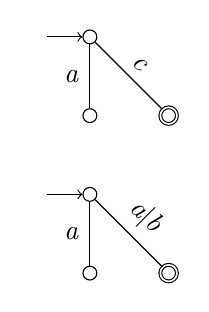
\begin{tikzpicture}
    \tikzstyle{every state}=[
        draw,
        shape=circle,
        inner sep=1pt,
        minimum size=5pt,
        final/.style={double,minimum size=6pt},
        initial text=]

    [->,auto]
    \renewcommand{\a}[1]{\textit{#1}}
    \node[state] [initial] (n0) {};
    \node[state] [below of=n0] (n1) {};
    \node[state, final] [right of=n1] (n3) {};
    \path (n0) edge node[left]{\a{a}} (n1)
            (n0) edge node[above=0mm,sloped]{\a{c}} (n3);

    \begin{scope}[yshift=-2cm]
    \node[state] [initial] (n0) {};
    \node[state] [below of=n0] (n1) {};
    \node[state, final] [right of=n1] (n3) {};
    \path (n0) edge node[left]{\a{a}} (n1)
            (n0) edge node[above=0mm,sloped]{$\a{a}|\a{b}$} (n3);
    \end{scope}
\end{tikzpicture}
\end{document}